\documentclass[a4paper,12pt]{article}
\usepackage[utf8]{inputenc}
\usepackage[spanish]{babel}
\usepackage{amsmath}
\usepackage{graphicx}
\usepackage{longtable}
\usepackage{amsfonts}
\usepackage{amssymb}
\usepackage[a4paper,margin=1in]{geometry}
\usepackage{fancyhdr}
\usepackage{titlesec}
\usepackage{titling}
\usepackage{xcolor}
\usepackage{booktabs}
\usepackage{float}

\usepackage{xcolor} % Paquete para colores
\usepackage{enumitem} % Paquete para personalizar listas

\usepackage[breaklinks=true]{hyperref}  % Permite el ajuste de los enlaces largos
\usepackage{url}  % Paquete para manejar URLs largas
\usepackage{breakurl}  % Paquete adicional para romper URLs
\usepackage{microtype}  % Mejora el ajuste del texto
\usepackage{microtype}
\def\UrlBreaks{\do\/\do-\do_\do.\do:\do\?}
\usepackage[backend=biber]{biblatex} % Paquete para gestionar las referencias\addbibresource{referencias.bib} 
\addbibresource{referencias.bib} % Añadir el archivo .bib


\begin{document}

\begin{titlepage}
    \centering
    \vspace*{1cm}
    \textbf{UNIVERSIDAD NACIONAL AUTÓNOMA DE MÉXICO}
    
    \vspace{0.5cm}
    \textbf{FACULTAD DE CIENCIAS, 2025-II}
    
    \vspace{0.5cm}
    \textbf{Organización y Arquitectura de Computadoras}
    
    \vspace{5 cm}
    \textbf{\LARGE \textcolor{teal}{TAREA 03:}}
    \vspace{1cm}\\
    \textbf{\LARGE \textcolor{teal}{Lógica digital}}
    \vspace{3cm}\\

    \Large Baños Mancilla Ilse Andrea - 321173988\\
    \vspace{1 cm}
    \Large Rivera Machuca Gabriel Eduardo 321057608
    
  
    \vspace{1cm}
\end{titlepage}

\section*{\textcolor{teal}{Preguntas}}

\begin{enumerate}[label=\textcolor{teal}{\textbf{\arabic*.}}]
%-------------Pregunta 1-------------------------------------------
    \item Demuestra que $x(yz)=(xy)z$ \\
    
        $x(xy) =(xy)z$ T6b\\

        $\therefore x(yz)=(xy)z$ 
%-------------Pregunta 2------------------------------------------- 
    \item Demuestra si la siguiente igualdad es válida $x(\overline{x}+y)=xy$ 
        
            


%-------------Pregunta 3-------------------------------------------
    \item  Demuestra si la siguiente igualdad es válida $(x+y)(\overline{x}+z)(y+z)=(x+y)(\overline{x}+z)$\\
    
        $(x+y)(\overline{x}+z)(y+z) $\\
        $= [(x+y)(\overline{x}+z)](y+z) $\\
        $= [(x+y)\overline{x} +(x+y)z](y+z) $ P4a\\
        $= [\overline{x}(x+y) +z(x+y)](y+z) $ P3b\\
        $= [(\overline{x}x+\overline{x}y) +(zx+zy)](y+z) $ P4a\\
        $= [(x \overline{x}+\overline{x}y) +(zx+zy)](y+z) $ P3b\\
        $= [(0+\overline{x}y) +(zx+zy)](y+z) $ P5b\\
        $= [\overline{x}y +zx+zy](y+z) $ P2a\\ 
        $= (\overline{x}y +zx+zy)y+(\overline{x}y +zx+zy)z $ P4a\\ 
        $= y(\overline{x}y +zx+zy)+z(\overline{x}y +zx+zy) $ P3b\\
        $= y\overline{x}y +yzx+yzy+z\overline{x}y +zzx+zzy $ P4a\\
        $= \overline{x}yy +yzx+yyz+yz\overline{x} +xzz+yzz $ P3b\\
        $= \overline{x}y +yzx+yz+yz\overline{x} +xz+yz $ T1b\\
        $= \overline{x}y +xz+yz+yz+ +yzx+yz\overline{x} $ P3a\\
        $= \overline{x}y +xz+yz +yzx+yz\overline{x} $  T1a\\
        $= \overline{x}y +xz+yz +yz(x+\overline{x}) $  P4a\\
        $= \overline{x}y +xz+yz +yz(1) $  P5a\\
        $= \overline{x}y +xz+yz +yz$  P2b\\
        $= \overline{x}y +xz+yz$  T1a\\
        $= 0 +\overline{x}y +xz+yz$  P2a\\
        $= x\overline{x} +\overline{x}y +xz+yz$  P5b\\
        $= \overline{x}x +\overline{x}y +zx+zy$  P3b\\
        $= \overline{x}(x +y) +z(x+y)$  P4a\\
        $= (x +y)\overline{x} +(x+y)z$  P3b\\
        $= (x +y)(\overline{x} +z)$  P4a\\

        $\therefore(x+y)(\overline{x}+z)(y+z)=(x+y)(\overline{x}+z)$\\

%-------------Pregunta 4-------------------------------------------            
    \item  Demuestra si la siguiente igualdad es válida $\overline{xy}=\overline{x} \cdot \overline{y}$
        
        
%-------------Pregunta 5-------------------------------------------

    \item Verifica la siguiente igualdad usando los postulados de Huntington
            \begin{center}
                $F(x,y,z) = x + x(\overline{x} + y) + \overline{x} y = x + y$
            \end{center}

            $x + x(\overline{x} + y) + \overline{x} y$\\
            $= x + x\overline{x} + xy + \overline{x} y$ P4a\\
            $= x + 0 + xy + \overline{x} y$ P5b\\
            $= x + xy + \overline{x} y$ P2a\\
            $= x + yx + y\overline{x} $ P3b\\
            $= x + y(x + \overline{x}) $ P4a\\
            $= x + y(1) $ P5a\\
            $= x + y $ P2b\\

            $ \therefore x + x(\overline{x} + y) + \overline{x} y = x + y$\\
           
%-------------Pregunta 6-------------------------------------------

    \item Obten los mintérminos y reduce la siguiente función 
        \begin{center}
            $F(x,y,z) = \overline{x} \cdot \overline{y} \cdot \overline{z} \cdot x + \overline{z} \cdot x + z \cdot x + x \cdot \overline{y} + \overline{z} $
        \end{center}
%-------------Pregunta 7-------------------------------------------

    \item Simplifica la siguiente función usando su tabla de verdad asociada y mapas de Karnaugh.
    
        \begin{center}
            $F(x,y,z) = \overline{xyz} + \overline{xy} z + \overline{x} y \overline{z} + x \overline{yz} +  \overline{x} yz +x \overline{y} z +xyz $
        \end{center}

        Tabla de verdad

        \begin{center}
            \begin{table}[h]
            \centering
            \begin{tabular}{|c|c|c|c|}
                \hline
                x & y & z & F \\ 
                \hline
                0 & 0 & 0 & 1 \\ 
                \hline 
                0 & 0 & 1 & 1 \\ 
                \hline 
                0 & 1 & 0 & 1 \\ 
                \hline 
                0 & 1 & 1 & 1 \\ 
                \hline 
                1 & 0 & 0 & 1 \\ 
                \hline 
                1 & 0 & 1 & 1 \\ 
                \hline 
                1 & 1 & 0 & 0 \\
                \hline 
                1 & 1 & 1 & 1 \\ 
                \hline 
            \end{tabular}\\
        \end{table}
        \end{center}

        Mapa de Karnaugh

        \begin{figure}[h]
            \centering
            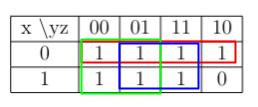
\includegraphics[width=5 cm]{img/mapa7.jpg}
        \end{figure}
        
        $ \therefore$ la expresión reducida es  $ \textcolor{red}{\overline{x}}+ \textcolor{green}{\overline{y}} + \textcolor{blue}{z}$

%-------------Pregunta 8-------------------------------------------
    \item Reduce la siguiente función y da sus maxitérminos
        \begin{center}
            $F(x,y,z) = (x + \overline{x} z) \cdot (\overline{y} + \overline{z}) z$
        \end{center}

%-------------Pregunta 9-------------------------------------------
    \item Utilizando Mapas de Karnaugh simplifica la función.\\
    
        \begin{center}
            $F(x_0,x_1,x_2,x_3) =
            \overline{x_0 x_1 x_2 x_3} 
            +\overline{x_0 x_1 x_2} x_3
            +\overline{x_0 x_1} x_2 x_3
            +x_0 \overline{x_1} x_2 x_3
            + x_0 x_1 \overline{x_2 x_3}
            + \overline{x_0} x_1 \overline{x_2 x_3}
            +x_0 x_1 x_2 x_3
            $
        \end{center}
        
        \begin{figure}[h]
            \centering
            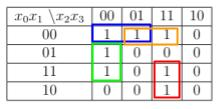
\includegraphics[width=5 cm]{img/mapa9.jpg}
        \end{figure}
        
        $ \therefore$ la expresión reducida es $\textcolor{red}{x_0 x_2 x_3} + \textcolor{green}{x_1 \overline{x_2 x_3}} + \textcolor{blue}{\overline{x_0 x_1 x_2}} + \textcolor{orange}{\overline{x_0 x_1} x_3}$

%-------------Pregunta 10-------------------------------------------
    \item Para realizar una Mapa de Karnaugh con más de 5 variables se mencionó que existe más de
    una forma de representarlo.\\
    Investiga ambos métodos y utiliza el que más se te acomode para reducir la siguiente función.

    \begin{center}
        $F(x_0,x_1,x_2,x_3,x_4) = 
        \overline{x_0 x_1 x_2 x_3 x_4} 
        + \overline{x_0 x_1 x_2} x_3 \overline{x_4} 
        + \overline{x_0 x_1} x_2 x_3 \overline{x_4} 
        + x_0 \overline{x_1} x_2 x_3 x_4
        + x_0 x_1 \overline{x_2 x_3} x_4
        + \overline{x_0} x_1 \overline{x_2 x_3} x_4
        + x_0 x_1 x_2 x_3 x_4 
        $
    \end{center}
   
%-------------Pregunta 11-------------------------------------------
    \item Utilizando el algoritmo de Quine-McCluskey realiza la siguiente reducción.

        \begin{center}
            $F(x_0,x_1,x_2,x_3,x_4) = 
            \overline{x_0 x_1 x_2 x_3 x_4} 
            + \overline{x_0 x_1 x_2} x_3 \overline{x_4} 
            + \overline{x_0} x_1 x_2 x_3 \overline{x_4}   
            + \overline{x_0} x_1 \overline{x_2} x_3 \overline{x_4}  
            + x_0 \overline{x_1} x_2 x_3 x_4    
            + x_0 x_1 \overline{ x_2 x_3} x_4 
            + \overline{x_0} x_1 \overline{ x_2 x_3} x_4 
            + x_0 x_1 x_2 \overline{ x_3} x_4 
            + x_0 x_1 x_2 x_3 x_4 
             $
        \end{center}

%-------------Pregunta 12-------------------------------------------
    \item Utilizando el algoritmo de Quine-McCluskey realiza la siguiente reducción.
        \begin{center}
            $F(x_0,x_1,x_2,x_3,x_4) = 
            \overline{x_0 x_1 x_2 x_3 x_4} 
            + \overline{x_0 x_1 x_2} x_3 \overline{x_4} 
            + \overline{x_0 x_1} x_2 x_3 \overline{x_4}  
            + \overline{x_0 x_1} x_2 x_3 x_4  
            + \overline{x_0} x_1 x_2 x_3 \overline{x_4} 
            + \overline{x_0} x_1 \overline{x_2} x_3 \overline{x_4} 
            + x_0 \overline{x_1} x_2 x_3 x_4
            + x_0 x_1 \overline{x_2 x_3} x_4
            + \overline{x_0} x_1 \overline{x_2 x_3} x_4
            + x_0 x_1 x_2 \overline{ x_3} x_4 
            + x_0 x_1 x_2 x_3 x_4 
            $
        \end{center}
    


\end{enumerate}


%--\nocite{*}
%--\printbibliography

\end{document}
